%%%%%%%%%%%%%%%%%%%%%%%%%%%%%%%%%%%%%%%%%%%%%%%%%%%%%%%%%%%%%%%%%%%%%%%%%%%%%%%%%%
\begin{frame}[fragile]\frametitle{}
\begin{center}
{\Large Differentiation}
\end{center}
\end{frame}


%%%%%%%%%%%%%%%%%%%%%%%%%%%%%%%%%%%%%%%%%%%%%%%%%%%%%%%%%%%
 \begin{frame}[fragile]\frametitle{Derivative}
Slope of a graph between a section (ie two points) can be easily calculated.
\begin{center}
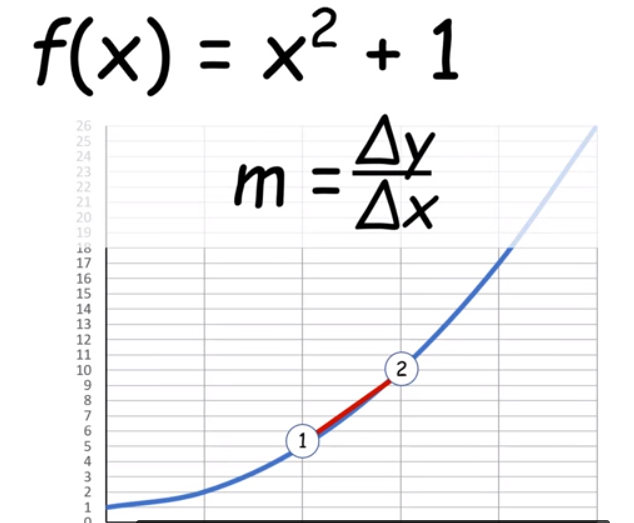
\includegraphics[width=0.5\linewidth,keepaspectratio]{diff1}
\end{center}

\end{frame}


%%%%%%%%%%%%%%%%%%%%%%%%%%%%%%%%%%%%%%%%%%%%%%%%%%%%%%%%%%%
 \begin{frame}[fragile]\frametitle{Derivative}
Delta x can be replaced by $h$ and the formula for segment slope becomes.
\begin{center}
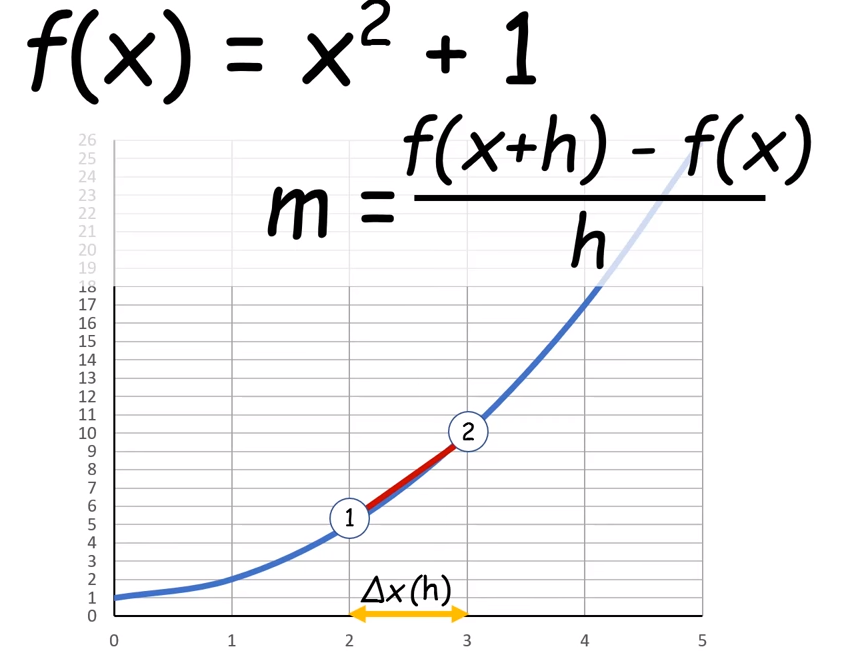
\includegraphics[width=0.5\linewidth,keepaspectratio]{diff2}
\end{center}

\end{frame}

%%%%%%%%%%%%%%%%%%%%%%%%%%%%%%%%%%%%%%%%%%%%%%%%%%%%%%%%%%%
 \begin{frame}[fragile]\frametitle{Derivative}
If both points come very close then we can say that the `Segment Slope' becomes a `Point Slope'.
\begin{center}
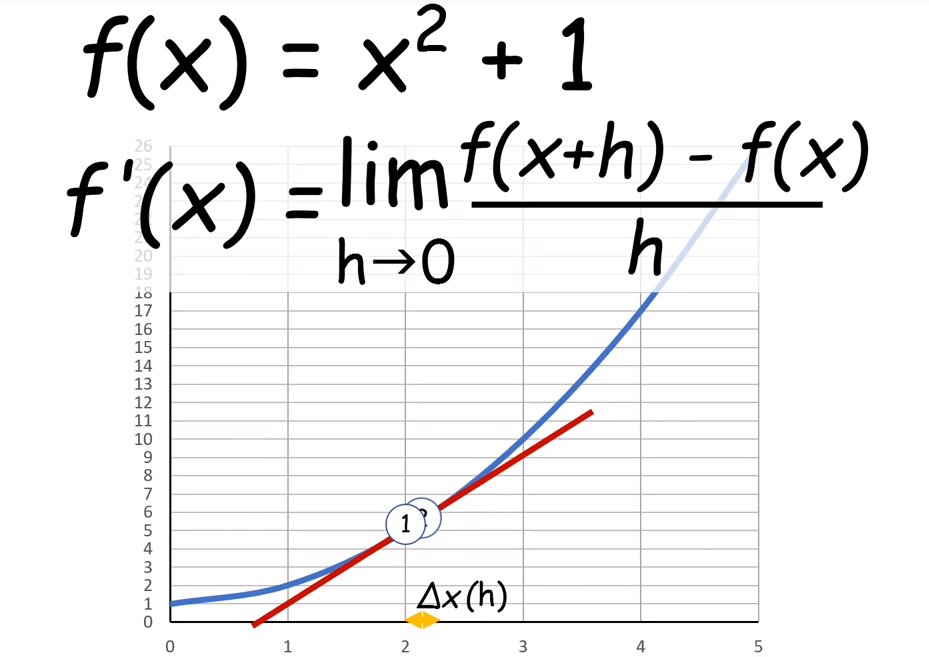
\includegraphics[width=0.5\linewidth,keepaspectratio]{diff3}
\end{center}
The concept of Limits is used to determine RATE OF CHANGE at a given POINT.

\end{frame}

%%%%%%%%%%%%%%%%%%%%%%%%%%%%%%%%%%%%%%%%%%%%%%%%%%%%%%%%%%%
 \begin{frame}[fragile]\frametitle{Derivative}
How to calculate value of the derivative at a points, say $x=3$?

\begin{center}
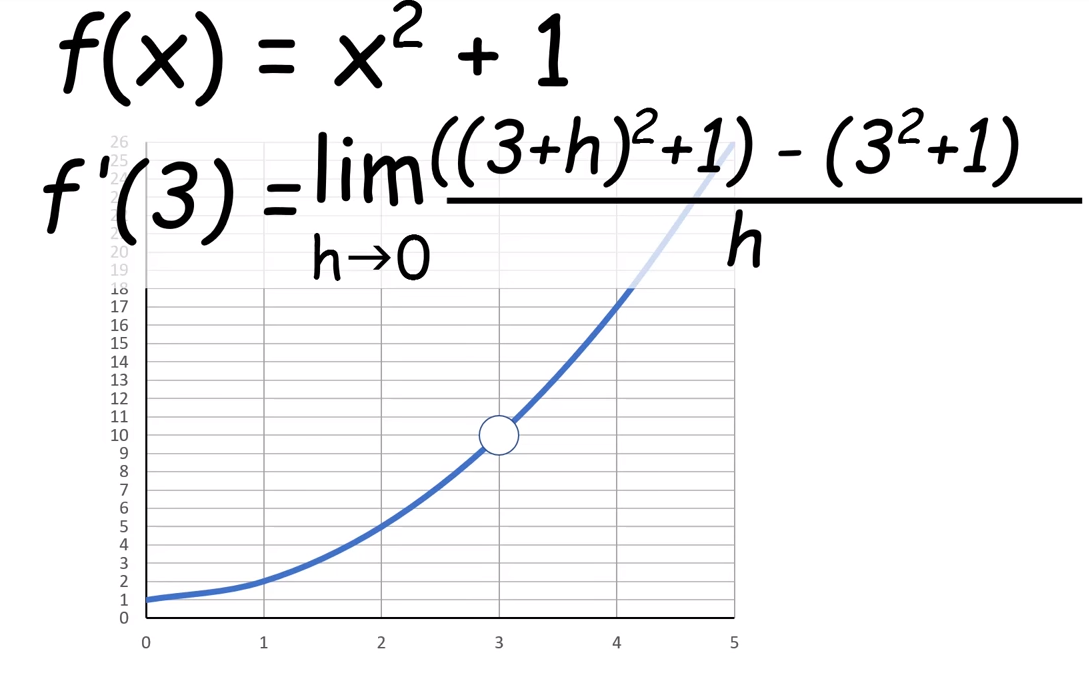
\includegraphics[width=0.5\linewidth,keepaspectratio]{diff4}
\end{center}

$f'(3) = 6$
\end{frame}

%%%%%%%%%%%%%%%%%%%%%%%%%%%%%%%%%%%%%%%%%%%%%%%%%%%%%%%%%%%
 \begin{frame}[fragile]\frametitle{Derivative}
\begin{itemize}
\item Slope at a point on curve is linear, where as the curve itself is not linear.
\item Tangent plane at a point on a sphere is linear but the sphere is not.
\item So, derivative is a Linear approximation
\end{itemize}
\end{frame}


%%%%%%%%%%%%%%%%%%%%%%%%%%%%%%%%%%%%%%%%%%%%%%%%%%%%%%%%%%%
 \begin{frame}[fragile]\frametitle{Differentiability}
\begin{itemize}
\item Note: A function may not be differentiable at every point; that is you might not be able to calculate the derivative for
every point on the function line. 
\item To be differentiable at a given point, the function must be continuous at that point, 
\item The tangent line at that point cannot be vertical, and the line must be smooth at that point 
\item Cannot suddenly change direction or have kinks
\end{itemize}
\end{frame}

%%%%%%%%%%%%%%%%%%%%%%%%%%%%%%%%%%%%%%%%%%%%%%%%%%%%%%%%%%%
 \begin{frame}[fragile]\frametitle{Continuous Functions}
\begin{itemize}
\item A function below is not defined at certain points ($x = 10$)
\item At certain point ($x = 7$), it is multi valued.
\item At certain point ($x = 17$), the slope is vertical, so not differentiable.
\item At certain point ($x = 4$), there is sudden change in direction, so not differentiable.
\end{itemize}
\begin{center}
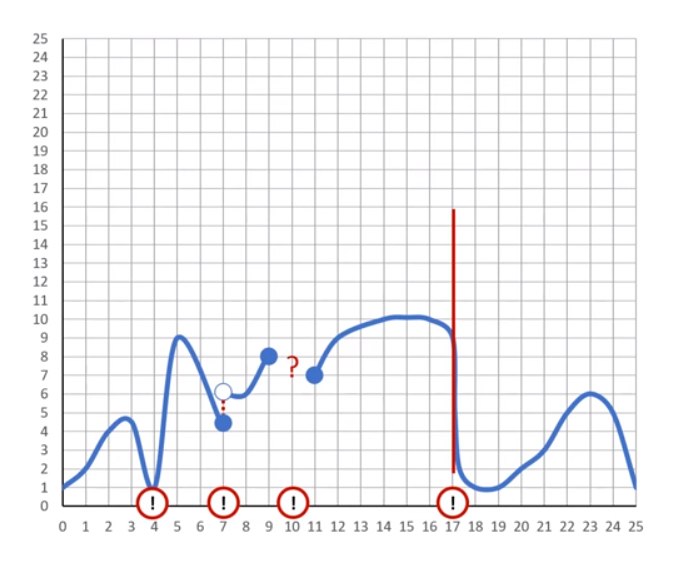
\includegraphics[width=0.5\linewidth,keepaspectratio]{diff5}
\end{center}
\end{frame}

%%%%%%%%%%%%%%%%%%%%%%%%%%%%%%%%%%%%%%%%%%%%%%%%%%%%%%%%%%%
 \begin{frame}[fragile]\frametitle{Continuous Functions}
\begin{itemize}
\item If two values are defined then all the values in between are defined.
\item Discontinuous functions: Step function: $f(x) = [x]$ integer part of x. This suddenly jumps from 0 to 1 to 2, etc.
\begin{center}
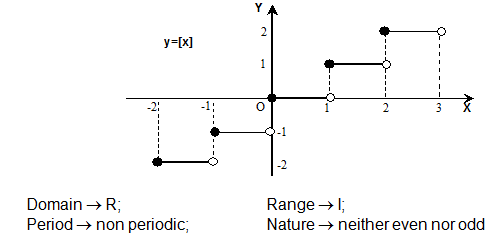
\includegraphics[width=0.8\linewidth,keepaspectratio]{step_range}
\end{center}
\end{itemize}
\end{frame}

%%%%%%%%%%%%%%%%%%%%%%%%%%%%%%%%%%%%%%%%%%%%%%%%%%%%%%%%%%%
 \begin{frame}[fragile]\frametitle{Differentiability}
\begin{itemize}
\item $f'(x_0) = \lim_{h \to 0} \frac{f(x_0 + h) - f(x_0)}{h} = A$ if limit exists.
\item In the above formula $x_0$ is constant, so this function is wrt $h$
\item So, $\lim_{h \to 0} g(h) = A$
\item For any given arbitrary $\epsilon > 0 $, there exists $\delta > 0$, so that if $0 < | h| < \delta$, then $|g(h) - A| < \epsilon$
\item However small $\epsilon$ can be made, we can still find corresponding $\delta$. The dependence is on $f$ as well as the point at which we are calculating.
\end{itemize}
\end{frame}

%%%%%%%%%%%%%%%%%%%%%%%%%%%%%%%%%%%%%%%%%%%%%%%%%%%%%%%%%%%
 \begin{frame}[fragile]\frametitle{Example}
\begin{itemize}
\item $f(x) = x^2$, at $x_0 = 1$
\item $f'(x) = \lim_{h to 0} \frac{(x+h)^2 - x^2}{h} = 2x + h$
\item Prove: $(x^n)' = n x^{n-1}$
\begin{align}
(x^n)'&=\lim_{h \to 0} {(x+h)^n-x^n\over h}\\
&=\lim_{h \to 0} {x^n+nx^{n-1}h+{n(n-1)\over 2}x^{n-2}h^2+\cdots+h^n-x^n\over h} \\
&=\lim_{h \to 0} \left[ nx^{n-1}+{n(n-1)\over 2}x^{n-2}h+\cdots+h^{n-1} \right]
\end{align}
\item $\lim_{h \to 0} \left[ nx^{n-1}+{n(n-1)\over 2}x^{n-2}h+\dots+h^{n-1} \right]= nx^{n-1}$
\end{itemize}
\end{frame}

%%%%%%%%%%%%%%%%%%%%%%%%%%%%%%%%%%%%%%%%%%%%%%%%%%%%%%%%%%%
 \begin{frame}[fragile]\frametitle{Example}
\begin{itemize}
\item $f(x) = x^2 + x $, at $x_0 = 5$
\item $f'(x) = \lim_{h \to 0} \frac{f(x + h) - f(x)}{h}$
\item $f'(x) = \lim_{h \to 0} \frac{((x+h)^{2} + x + h) - (x^{2} + x)}{h}$
\item $f'(x) = \lim_{h \to 0} \frac{x^{2} + h^{2} + 2xh + x + h - x^{2} - x}{h}$
\item $f'(x) = \lim_{h \to 0} 2x + h + 1 $
\item Evaluating the limit, ie $h=0$, becomes $f'(x) = 2x + 0 + 1$
\item For $x = 5 $ the result is $f'(5) = 2\cdot5 + 1 = 10 + 1 = 11$
\end{itemize}
\end{frame}

%%%%%%%%%%%%%%%%%%%%%%%%%%%%%%%%%%%%%%%%%%%%%%%%%%%%%%%%%%%
 \begin{frame}[fragile] \frametitle{Finding Tangent Lines}

The tangent line to \ $y=f(x)$ \ through\ $P$ \ is equal to \\
 \begin{center}
  {\bf the limit line of sequence { $\overset{\longleftrightarrow}{PQ_n}$. }}
 \end{center}

Thus,

\[ \text{\bf the slope of tangent line at\ $P$} \ = \lim_{n\to \infty} \; { \text{\bf the slope of} \; \overset{\longleftrightarrow}{PQ_n}}\]

\end{frame}

%%%%%%%%%%%%%%%%%%%%%%%%%%%%%%%%%%%%%%%%%%%%%%%%%%%%%%%%%%%
 \begin{frame}[fragile] \frametitle{Finding Tangent Lines}
\begin{align*}
 f'(a) :=& \;\text{\bf the slope of tangent line at\ $P(a,f(a))$}\\
 =& \lim_{x \to a}\; \frac{f(x)-f(a)}{x-a} \\
 =& \lim_{\Delta x \to 0}\; \frac{f(a+\Delta x)-f(a)}{\Delta x}
\end{align*}

Fine an equation of the tangent line to the parabola \ $y=x^2$\ at the point\ $P(1,1)$.
\end{frame}

%%%%%%%%%%%%%%%%%%%%%%%%%%%%%%%%%%%%%%%%%%%%%%%%%%%%%%%%%%%
 \begin{frame}[fragile] \frametitle{Differential functions}
A function \ $f=f(x)$\ having a derivative at\ $x=a$\ is also called {\bf differentiable} at \ $x=a$, i.e.
{\[f'(x) := \lim_{x\to a} \; \frac{f(x+\Delta x)-f(x)}{\Delta x} .\]}
 If it is differentiable at each point of\ $I$, is called {\bf differentiable on \ $I$}. 
The function\ $f' = f'(x)$\ is its {\bf differential function}.

Let\ $f(x)=x^3-x$, find a formula for\ $f'(x)$.

Let\ $f(x)=\sqrt{x-1}$. Find the derivative of\ $f$. State the domain of\ $f'$.

\end{frame}

%%%%%%%%%%%%%%%%%%%%%%%%%%%%%%%%%%%%%%%%%%%%%%%%%%%%%%%%%%%
 \begin{frame}[fragile] \frametitle{Differentiability implies Continuity}

	Where is the function\ $f(x)=|x|$\ differentiable?

If\ $f$\ is differentiable at\ $a$, then\ $f$\ is continuous at\ $a$.

\end{frame}

\newcommand \derv [1] {\frac{d {#1} }{d x}}
\newcommand \dderv [1] {\frac{d^2 {#1} }{d x^2}}




%%%%%%%%%%%%%%%%%%%%%%%%%%%%%%%%%%%%%%%%%%%%%%%%%%%%%%%%%%%
 \begin{frame}[fragile] \frametitle{Differentiation formulas}
Let\ $f=f(x)$\ and\ $g=g(x)$\ have derivatives at\ $x=a$. Then
\begin{itemize}
	\item $(f+g)'(a) = f'(a) + g'(a)$\\
	\item $(f-g)'(a) = f'(a) - g'(a)$\\
	\item $(fg)'(a) = f'(a)g(a) + f(a)g'(a)$\\
	\item$\big( \dfrac{f}{g} \big)'(a) = \dfrac{f'(a)g(a) - f(a)g'(a)}{[g(a)]^2}$
\end{itemize}

In general, the derivative\ $f'(a)$\  may be used by other notations:
\[ D f(a) \qquad \derv{} f(a) \qquad \derv f(a) \qquad \derv f \mid_{x=a} \quad D f \mid_{x=a} \]

If\ $h(x)=x g(x)$ and it is known that\ $g(3)=5$\ and\ $g'(3)=2$, find\ $h'(3)$.

\end{frame}

%%%%%%%%%%%%%%%%%%%%%%%%%%%%%%%%%%%%%%%%%%%%%%%%%%%%%%%%%%%
 \begin{frame}[fragile] \frametitle{Theorems}
Let\ $f$\ and\ $g$\ be differentiable on\ $I$, then so are the following functions. Moreover,
\begin{itemize}
	\item $(f+g)' = f' + g'$\\
	\item $(f-g)' = f' - g'$\\
	\item $(fg)' = f'g + fg'$\\
	\item $\big( \dfrac{f}{g} \big)' = \dfrac{f'g - fg'}{g^2}$
\end{itemize}

\textbf{The Power Rule}
\[ \derv {x^n} = n x^{n-1}, \quad \text{for any\ } n\in \mathbb R \]



 Fine an equation of the tangent line to the curve \ $y=x \sqrt x$\ at the point\ $(1,1)$. 


\end{frame}


%%%%%%%%%%%%%%%%%%%%%%%%%%%%%%%%%%%%%%%%%%%%%%%%%%%%%%%%%%%
 \begin{frame}[fragile] \frametitle{Examples}

\begin{itemize}
	\item $\derv{} (x^8+12x^5-4x^4+10 x^3-6x+5)$\ = ?\\
	\item Differentiate the function\ $f(t)=\sqrt t (1-t)$.  
	\item Find the points on the curve\ $y=x^4-6x^2+4$\ where the tangent line is horizontal. 
	\item Let\ $y=\dfrac{x^2+x-2}{x^3+6}$. Find\ $y'$\ =?\\
	\item Fine an equation of the tangent line to the curve \ $y=\dfrac{\sqrt x}{1+x^2}$\ at the point\ $(1,\dfrac{1}{2})$.  
\end{itemize}
\end{frame}

%%%%%%%%%%%%%%%%%%%%%%%%%%%%%%%%%%%%%%%%%%%%%%%%%%%%%%%%%%%
 \begin{frame}[fragile] \frametitle{Derivatives of trigonometric functions}

\begin{columns}[t]
\column{4.5cm}
1.\; $\derv{} (\sin x) = \cos x$ \\
3.\; $\derv{} (\tan x) = \sec^2 x$ \\
5.\; $\derv{} (\sec x) = \tan x \ \sec x$

\column{4.5cm}
2.\ $\derv{} (\cos x) = - \sin x$ \\
4.\ $\derv{} (\cot x) = - \csc^2 x$ \\
6.\ $\derv{} (\csc x) = - \cot x \ \csc x$
\end{columns}


\textbf{Proof for $\derv{} (\sin x) = \cos x$ }
\begin{align*}
\derv{\ \sin x}\mid_{x= a} &= \lim_{\Delta x \to 0} \frac{\sin (a+\Delta x) - \sin a}{\Delta x} \\
 &= \lim_{\Delta x \to 0} \frac{2 \cos (a+\frac{1}{2}\Delta x)\cdot \sin (\frac{1}{2}\Delta x) } {\Delta x} \\
 &= \cos a \cdot \lim_{\Delta x \to 0} \frac{\sin (\frac{1}{2}\Delta x)}{\frac{1}{2}\Delta x} = \cos a 
\end{align*}


\end{frame}

%%%%%%%%%%%%%%%%%%%%%%%%%%%%%%%%%%%%%%%%%%%%%%%%%%%%%%%%%%%
 \begin{frame}[fragile] \frametitle{Derivatives of trigonometric functions}
\begin{itemize}
  \item Find\ $\lim\limits_{x\to 0} \dfrac{\sin 7x}{4x}$.
	\item Calculate\ $\lim\limits_{x\to 0}\ x\cot x$.  
	\item Differentiate\ $y=x^2 \sin x$.  
	\item Differentiate\ $f(x)=\dfrac{\sec x}{1+\tan x}$.		
\end{itemize}
\end{frame}

%%%%%%%%%%%%%%%%%%%%%%%%%%%%%%%%%%%%%%%%%%%%%%%%%%%%%%%%%%%
 \begin{frame}[fragile] \frametitle{The chain rule}
Let\ $g=g(x)$\ be a differentiable function at\ $a$, and $f=f(x)$\ differentiable at\ $g(a)$. Then the composite function\ $f\circ g$ is differentiable at\ $a$, and
{\[ (f\circ g)'(a) = f'(g(a)) g'(a) .\]}
In Leibniz notation, let\ $y=f(u)$\ and\ $u=g(x)$\ be both differentiable, then
{\[\derv y = \frac{d y}{d u} \cdot \derv u \]}
\end{frame}

%%%%%%%%%%%%%%%%%%%%%%%%%%%%%%%%%%%%%%%%%%%%%%%%%%%%%%%%%%%
 \begin{frame}[fragile] \frametitle{}

$\derv y = \frac{d y}{d u} \cdot \derv u $

\begin{itemize}
	\item Find\ $f'(x)$\ if \ $f(x)=\sqrt{x^2+1}$. \\
	\item Differentiate\; (a)\ $y=\sin (x^2)$ \quad  (b)\ $y=\sin^2 x$.
	\item Differentiate\ $f'(x)$\ if \ $f(x)=(x^3-1)^{100}$. \\
	\item Find\  $f'(x)$\ if \ $f(x)=\dfrac{1}{\sqrt[3]{x^2+x+1}}$. 
\end{itemize}


\begin{itemize}
	\item Find the derivative of\; $g(t)= \big( \dfrac{t-2}{2t+1} \big)^9$.\\4[pt]
	\item Differentiate\; $y=(2x+1)^5(x^3-x+1)^4$. \\
	\item Find\  $f'(x)$\ if \ $f(x)=\sin \big( \cos ( \tan x ) \big)$. 
	\item Differentiate\; $y=\sqrt{\sec x^3}$.	
\end{itemize}


\end{frame}

%%%%%%%%%%%%%%%%%%%%%%%%%%%%%%%%%%%%%%%%%%%%%%%%%%%%%%%%%%%
 \begin{frame}[fragile] \frametitle{Differentials}

Let\ $y=y(u)$. The {\bf differential}\ $d {y}$\ is defined in terms of\ $d u$\ by the equation
{\[d y = y'(u)\, d u\]}
Moreover, if\ $u=u(x)$\ then
{ \[ d u = u'(x)\, d x \quad \text{and} \quad d y = y'(u)\, d u = y'(x) u'(x)\, d x \]}
\end{frame}

%%%%%%%%%%%%%%%%%%%%%%%%%%%%%%%%%%%%%%%%%%%%%%%%%%%%%%%%%%%
 \begin{frame}[fragile] \frametitle{Linear Approximations}
Let\ $f=f(x)$. The {\bf linear approximation} of\ $f$\ at\ $a$\ is the approximation
{\begin{align*}
 f(x) &\approx f(a) + f'(a) \Delta x \\
 &=f(a)+ f'(a)(x-a)
\end{align*}
} That means\ $\Delta f \approx df$.

\begin{itemize}
	\item Find the linearization of\ $f(x)=\sqrt{x+3}$\ at\ $a=1$\ and use it to approximate\ $\sqrt{3.98}$\ and\ $\sqrt{4.05}$.  
	\item Compare the values of\ $\Delta y$\ and\ $dy$\ if\ $y=f(x)=x^3+x^2-2x+1$
	and\ $x$\ changes (a) from 2 to 2.05 and (b) from 2 to 2.01.
\end{itemize}

\end{frame}

%%%%%%%%%%%%%%%%%%%%%%%%%%%%%%%%%%%%%%%%%%%%%%%%%%%%%%%%%%%
 \begin{frame}[fragile] \frametitle{Related Rates}

\begin{itemize}
	\item Air is being pumped into a spherical balloon so that its volume increases at a rate of 100 ${\rm cm}^3$/s. How fast is the radius of the balloon increasing when the diameter is 50 cm?
	\item Car A is traveling west at 50 mi/h and car B is traveling north at 60 mi/h. Both are headed for the intersection of the two roads. At what rate are the cars approaching each other when car A is 0.3 mi and car B is 0.4 mi from the intersection?  
\end{itemize}
\end{frame}

%%%%%%%%%%%%%%%%%%%%%%%%%%%%%%%%%%%%%%%%%%%%%%%%%%%%%%%%%%%
 \begin{frame}[fragile] \frametitle{Implicit differentiation}

\begin{itemize}
	\item If\ $x^2+y^2=25$, find\ $\derv y$.
	\item Find an equation of the tangent to the circle\ $x^2+y^2=25$\ at the point (3,4).
\end{itemize}



\begin{align*}
 &\derv{} (x^2+y^2) = \derv{} (25) \\
 &2x \derv x + 2y \derv y = 0  \\
 &\derv y \mid_{(3,4)} = - \dfrac {x}{y} \mid_{(3,4)} = - \frac{3}{4}
\end{align*}

\end{frame}

%%%%%%%%%%%%%%%%%%%%%%%%%%%%%%%%%%%%%%%%%%%%%%%%%%%%%%%%%%%
 \begin{frame}[fragile] \frametitle{Implicit differentiation}

\begin{itemize}
	\item Find\ $y'$\ if\ $x^3+y^3=6xy$.
	\item Find the tangent to the folium of Descartes\; $x^3+y^3=6xy$\ at the point (3,3).
	\item At what points on the curve is the tangent line horizontal?
\end{itemize}


Find\ $y'$\ if\ $\sin (x+y) = y^2 \cos x$.
\end{frame}

%%%%%%%%%%%%%%%%%%%%%%%%%%%%%%%%%%%%%%%%%%%%%%%%%%%%%%%%%%%
 \begin{frame}[fragile] \frametitle{Higher derivatives}
Let\ $f=f(x)$. If its derivative function\ $f'=f'(x)$\ has derivative, denoted by
{\[ f''(x) = \derv{} (\derv f) = \dderv f = D^2 f(x),\]}
then it is called the {\bf second derivative} of\ $f$.

Similarly, we define the {\bf third derivative} of\ $f$\ as
{\[ y'''=f'''(x)=\derv{} (\dderv y)=\frac{d^3 y}{dx^3} = D^3f(x)\]}
and {higher derivative} as
{\[ y^{(n)}=f^{(n)}=\frac{d^n y}{dx^n} = D^n f(x)\]}
\end{frame}

%%%%%%%%%%%%%%%%%%%%%%%%%%%%%%%%%%%%%%%%%%%%%%%%%%%%%%%%%%%
 \begin{frame}[fragile] \frametitle{example}
\begin{itemize}
	\item If\ $f(x)=x \cos x$, find and interpret\ $f''(x)$.
	\item Find all $n$-th derivatives of\ $y=x^3-6x^2-5x+3$.\\
	\item If\ $f(x)=\dfrac{1}{x}$, find\ $f^{(n)}(x)$. 
	\item Find\ $y'''$\ if\ $x^4+y^4=16$.  \\
	\item Find\ $f^{(27)}$\ if\ $f(x)=\cos x$.
\end{itemize}
\end{frame}

%%%%%%%%%%%%%%%%%%%%%%%%%%%%%%%%%%%%%%%%%%%%%%%%%%%%%%%%%%%
 \begin{frame}[fragile] \frametitle{Analyzing Functions using Derivatives}
 Both Function and its Derivative is plotted.
\begin{center}
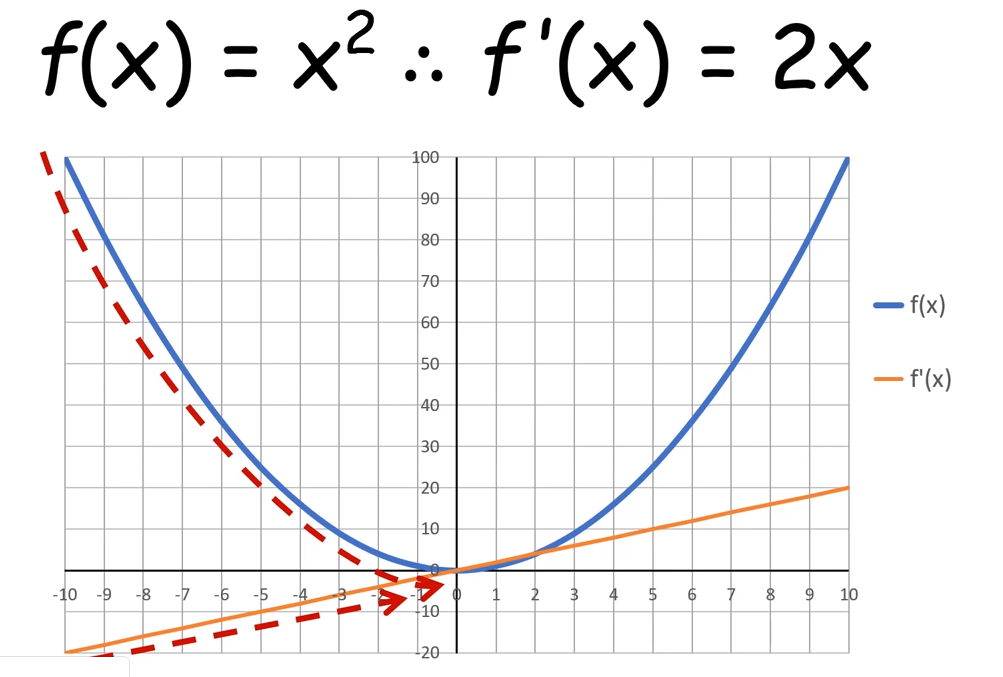
\includegraphics[width=0.5\linewidth,keepaspectratio]{diff6}
\end{center}
As we come from left hand side, the function value is reducing. Derivative values is decreasing form higher negative values to lesser negative values, approaching 0.
\end{frame}

%%%%%%%%%%%%%%%%%%%%%%%%%%%%%%%%%%%%%%%%%%%%%%%%%%%%%%%%%%%
 \begin{frame}[fragile] \frametitle{Analyzing Functions using Derivatives}
After crossing the min point of function, where derivative is 0, the derivative starts increasing as well as the function.
\begin{center}
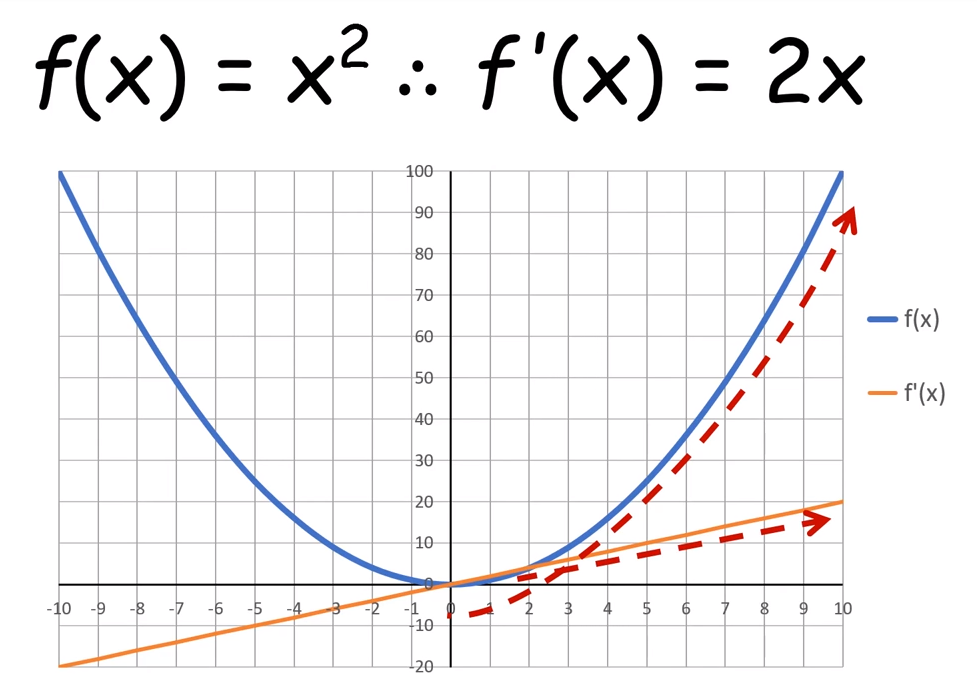
\includegraphics[width=0.5\linewidth,keepaspectratio]{diff7}
\end{center}
The derivative changeover point is potentially maximal or minimal point.
\end{frame}

%%%%%%%%%%%%%%%%%%%%%%%%%%%%%%%%%%%%%%%%%%%%%%%%%%%%%%%%%%%%%%%%%%%%%%%%%%%%%%%%%%
\begin{frame}[fragile]\frametitle{}
\begin{center}
{\Large 2nd order Derivative}
\end{center}
\end{frame}



%%%%%%%%%%%%%%%%%%%%%%%%%%%%%%%%%%%%%%%%%%%%%%%%%%%%%%%%%%%
 \begin{frame}[fragile] \frametitle{2nd order differentiation}

\begin{itemize}
	\item Finding rate of change of rate of change !!
	\item Velocity is rate of change of Distance
	\item Whats rate of change of Velocity?
	
\end{itemize}
Need 2nd order derivative in finding type of point where derivative goes 0, ie maxima or minima.

\end{frame}

%%%%%%%%%%%%%%%%%%%%%%%%%%%%%%%%%%%%%%%%%%%%%%%%%%%%%%%%%%%
 \begin{frame}[fragile] \frametitle{Maxima or Minima}

\begin{center}
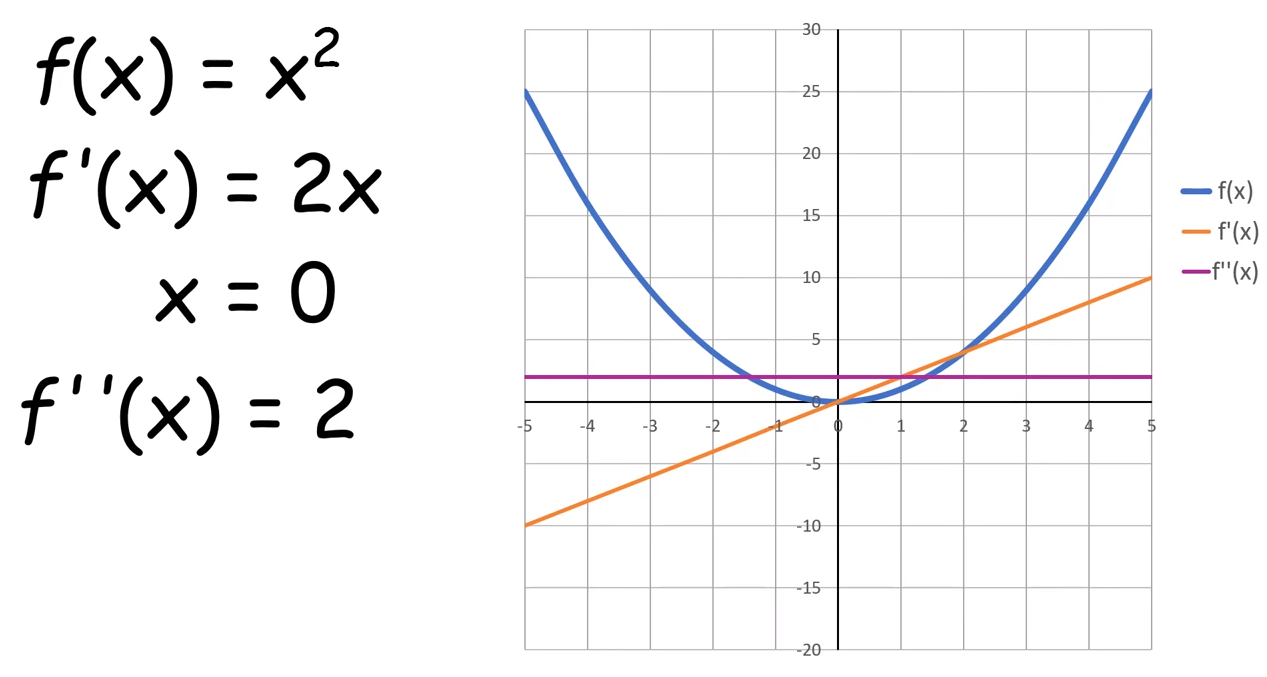
\includegraphics[width=0.5\linewidth,keepaspectratio]{diff8}
\end{center}

The derivative itself is a function. Its 2nd order derivative is coming to be a constant $+2$. 
So first order derivative is crossing from negative to positive. Thus its a Minima point.
\end{frame}

%%%%%%%%%%%%%%%%%%%%%%%%%%%%%%%%%%%%%%%%%%%%%%%%%%%%%%%%%%%
 \begin{frame}[fragile] \frametitle{Maxima or Minima}

\begin{center}
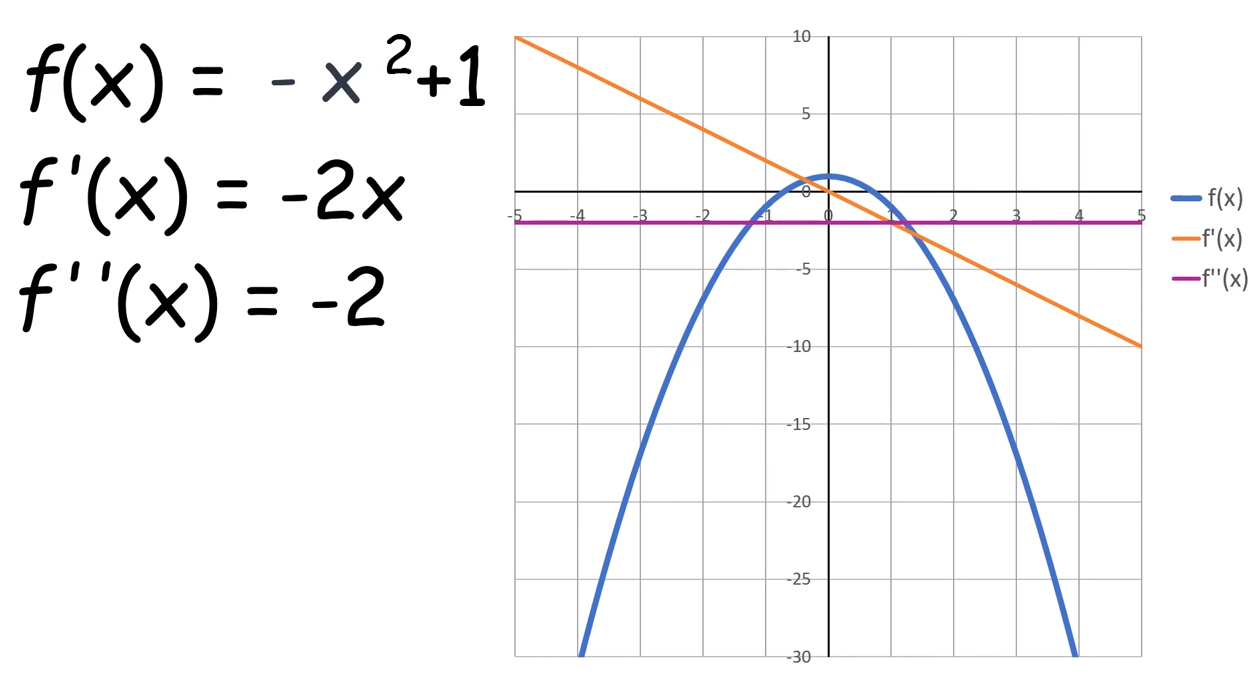
\includegraphics[width=0.5\linewidth,keepaspectratio]{diff9}
\end{center}

Its 2nd order derivative is coming to be a constant $-2$. 
So first order derivative is crossing from positive to negative. Thus its a Maxima point.
\end{frame}


%%%%%%%%%%%%%%%%%%%%%%%%%%%%%%%%%%%%%%%%%%%%%%%%%%%%%%%%%%%
 \begin{frame}[fragile] \frametitle{Optimization}

\begin{center}
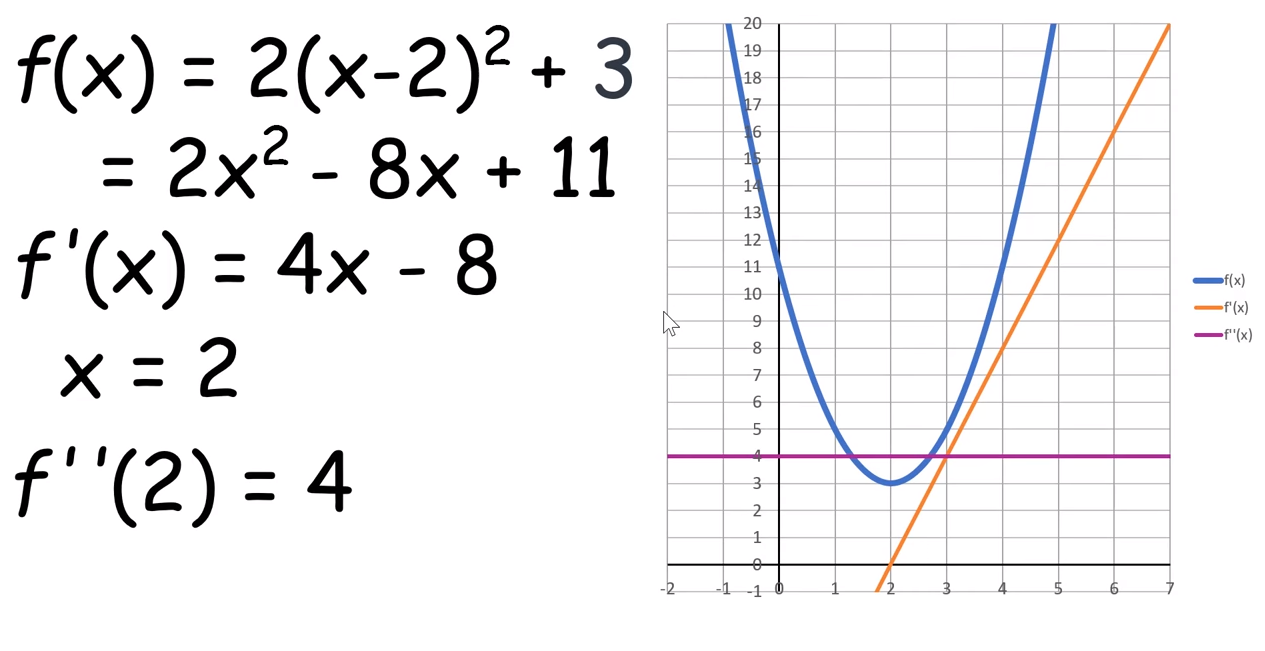
\includegraphics[width=0.5\linewidth,keepaspectratio]{diff10}
\end{center}
First derivative goes to 0 at $x=2$. At that point second derivative is positive. Thus its a Minima point.

\end{frame}









%%%%%%%%%%%%%%%%%%%%%%%%%%%%%%%%%%%%%%%%%%%%%%%%%%%%%%%%%%%%%%%%%%%%%%%%%%%%%%%%%%
\begin{frame}[fragile]\frametitle{}
\begin{center}
{\Large Partial Derivative}
\end{center}
\end{frame}


%%%%%%%%%%%%%%%%%%%%%%%%%%%%%%%%%%%%%%%%%%%%%%%%%%%%%%%%%%%
 \begin{frame}[fragile] \frametitle{Partial Derivative}
\begin{itemize}
\item Functions can be of more-than-one-variable, say two variables: x and y. 
\item When plotted it will be 3D plot. 2 input variables and 1 output variable, total 3.
\item For finding derivatives of such functions: we do it turn by turn. 
\item First wrt x then wrt y and so on. While taking derivative wrt x, the y is considered as constant.
\end{itemize}
\begin{center}
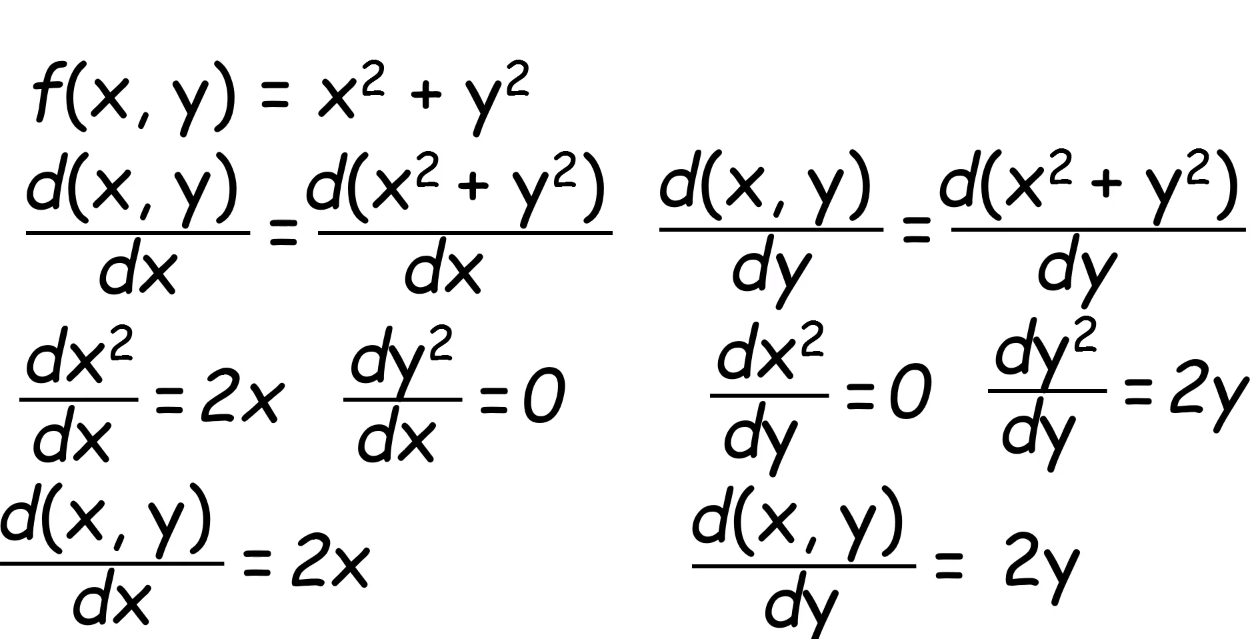
\includegraphics[width=0.5\linewidth,keepaspectratio]{diff11}
\end{center}
\end{frame}


%%%%%%%%%%%%%%%%%%%%%%%%%%%%%%%%%%%%%%%%%%%%%%%%%%%%%%%%%%%
\begin{frame}[fragile]\frametitle{}
\textbf{Definition}
 Suppose that $f(x,y)$ is a function of two variables with domain $D$.  Suppose that $(a,b)\in D$.  Define $g(x)=f(x,y)$ and $h(y)=f(x,y)$.  Then we define the \underline{partial derivatives of $f$ with} \underline{respect to the variables $x$ and $y$} as follows.
 $$
 f_x(x,y) = g'(x), \qquad f_y(x,y) = h'(y).
 $$


\textbf{Fact}
\begin{eqnarray*}
  f_x(a,b) &=& \lim_{h\rightarrow 0} \frac{f(a+h,b)-f(a,b)}{h}    \quad \mbox{and} \\
  f_y(a,b) &=& \lim_{h\rightarrow 0} \frac{f(a,b+h)-f(a,b)}{h}.
\end{eqnarray*}  
 
\end{frame}


%%%%%%%%%%%%%%%%%%%%%%%%%%%%%%%%%%%%%%%%%%%%%%%%%%%%%%%%%%%
\begin{frame}[fragile]\frametitle{}
\textbf{Notation}
\begin{eqnarray*}
  f_x(x,y) &=&  f_x = \frac{\partial f}{\partial x} = \frac{\partial}{\partial x} f(x,y) = \frac{\partial z}{\partial x}= f_1 = D_1 f= D_x f, \\
  f_y(x,y) &=&  f_y = \frac{\partial f}{\partial y} = \frac{\partial}{\partial y} f(x,y) = \frac{\partial z}{\partial y}= f_2 = D_2 f= D_y f. 
\end{eqnarray*}
  

\textbf{Example}
 Compute the partial derivatives with respect to $x$ and $y$ for the following functions.
\begin{enumerate}
  \item  $f(x,y) = x^4 + y^3 + 3xy$.
  \item $g(x,y) = \sin(xy)$.
\end{enumerate}

\end{frame}


%%%%%%%%%%%%%%%%%%%%%%%%%%%%%%%%%%%%%%%%%%%%%%%%%%%%%%%%%%%
\begin{frame}[fragile]\frametitle{}
\textbf{Note}
 Suppose that $f(x,y)$ is a function with domain $D$ and that $(a,b)\in D$.  Consider the curves $C_x : z= f(x,b)$  and $C_y : z=f(a,y)$.  The slope of the line in the plane $y=b$ which is tangent to $C_x$ at $(a,b,(f(a,b))$ is $f_x(a,b)$.  \\ 
 The slope of the line in the plane $x=a$ which is tangent to $C_y$ at $(a,b,f(a,b))$ is $f_y(a,b)$.  \\ 
 The equations of the tangent lines are 
 \begin{eqnarray*}
 \begin{cases} z-c= f_x(a,b) (x-a) \\  y=b.\end{cases} \quad \begin{cases} z-c= f_y(a,b)(y-b) \\ x=a. \end{cases}
 \end{eqnarray*}  
 They can be parametrized by the vector functions
   \begin{eqnarray*}
      r_x(t) &=& (a,b,c) + t(1,0,f_x(a,b)) \quad \mbox{and}  \\
      r_y(t) &=& (a,b,c) + t(0,1,f_y(a,b)).
    \end{eqnarray*}
 
\end{frame}


%%%%%%%%%%%%%%%%%%%%%%%%%%%%%%%%%%%%%%%%%%%%%%%%%%%%%%%%%%%
\begin{frame}[fragile]\frametitle{}
\textbf{Example}
\begin{enumerate}
  \item Find the equations of the tangent lines to the graph of $f(x,y)= \sin(xy)$ at the point $(\pi,\frac{1}{2},1)$.  
  \item  Find the equations of the tangent lines to the sphere $x^2+y^2+z^2=9$  at the point $(\sqrt{3},\sqrt{3},\sqrt{3})$. 
\end{enumerate}

\end{frame}



%%%%%%%%%%%%%%%%%%%%%%%%%%%%%%%%%%%%%%%%%%%%%%%%%%%%%%%%%%%
\begin{frame}[fragile]\frametitle{}
\textbf{Note}
 We can of course consider the partial derivatives of functions of many variables.  Suppose that $f(\vec{x})$ is a function of the $n$ variables $x_1, \dots, x_n$.  Then we define 
 $$f_{x_i}(\vec{a}) = \lim_{h\rightarrow 0} \frac{f(a_1, \dots, a_{i-1}, a_i+h, a_{i+1}, \dots, a_n) - f(a_1,\dots, a_n)}{h}.$$
 We can of course use the rules of differentiating functions of one variable to compute these partials.
  

\textbf{Example}
 Compute the partial derivatives of $f(x,y,z) = x\sin(y)e^z$.

\end{frame}



%%%%%%%%%%%%%%%%%%%%%%%%%%%%%%%%%%%%%%%%%%%%%%%%%%%%%%%%%%%
\begin{frame}[fragile]\frametitle{}
\textbf{Note}
 We can of course consider higher derivatives.  The notation for the second order derivatives is as follows.
 \begin{eqnarray*}
 (f_x)_x &=& f_{xx} = \frac{\partial}{\partial x}\left( \frac{\partial f}{\partial x}\right) = \frac{\partial^2 f}{{\partial x}^2},  \\
 (f_x)_y &=& f_{xy} = \frac{\partial}{\partial y}\left( \frac{\partial f}{\partial x}\right) = \frac{\partial^2 f}{\partial y \partial x},  \\
 (f_y)_x &=& f_{yx} = \frac{\partial}{\partial x}\left( \frac{\partial f}{\partial y}\right) = \frac{\partial^2 f}{\partial x \partial y},  \\
 (f_y)_y &=& f_{yy} = \frac{\partial}{\partial y}\left( \frac{\partial f}{\partial y}\right) = \frac{\partial^2 f}{{\partial y}^2}.  \\
 \end{eqnarray*} 
 The notation for third and higher order derivatives is similar.

\end{frame}


%%%%%%%%%%%%%%%%%%%%%%%%%%%%%%%%%%%%%%%%%%%%%%%%%%%%%%%%%%%
\begin{frame}[fragile]\frametitle{}
\textbf{Example}
 Let $f(x,y) = x^2 -xy +y^2$.  Compute the 2nd order partial derivatives of $f$.
  

\textbf{Theorem}[Clairaut]
 Suppose that $f$ is defined at $(a,b)$.  If there is a disk $D$ containing $(a,b)$ on which $f_{xy}$ and $f_{yx}$ are continuous, then 
 $$f_{xy}(a,b)=f_{yx}(a,b).$$

\end{frame}



%%%%%%%%%%%%%%%%%%%%%%%%%%%%%%%%%%%%%%%%%%%%%%%%%%%%%%%%%%%
\begin{frame}[fragile]\frametitle{}
 \textbf{Fact}
   Suppose that $f$ has continuous partial derivatives at $(x_0,y_0)$.  Then the \underline{tangent plane of $f$ at $(x_0,y_0)$} (i.e. the plane determined by the tangent lines to $z=f(x,y)$ at $(x_0,y_0,f(x_0,y_0))$. has the equation
   $$
     z-f(x_0,y_0) = f_x(x_0,y_0)(x-x_0) + f_y(x_0,y_0)(y-y_0).
   $$
  

\textbf{Example}
  Find the equation of the plane tangent to $z=3x^2+5y^2$ at the point $(1,1,8)$.

\end{frame}


%%%%%%%%%%%%%%%%%%%%%%%%%%%%%%%%%%%%%%%%%%%%%%%%%%%%%%%%%%%
 \begin{frame}[fragile] \frametitle{Gradient}

\begin{enumerate}
  \item Partial derivatives are important if you want to find the analog of the slope for multi-dimensional surfaces. We call this quantity the gradient.
 \item For $f(x,y) = x^2 + y^2$ the partial derivatives are:
 \begin{align}
 \frac{\partial f(x,y)}{\partial x} = 2x \\
\frac{\partial f(x,y)}{\partial y} = 2y
\end{align}
\item The Gradient
\begin{eqnarray*}
grad(f(x,y)) =  \vec{g(x,y)} = \begin{bmatrix}\frac{\partial f(x,y)}{\partial x} \\ \frac{\partial f(x,y)}{\partial y} \end{bmatrix} = \begin{bmatrix}2x \\ 2y \end{bmatrix}
\end{eqnarray*}

\end{enumerate}
 

\end{frame}

%%%%%%%%%%%%%%%%%%%%%%%%%%%%%%%%%%%%%%%%%%%%%%%%%%%%%%%%%%%
 \begin{frame}[fragile] \frametitle{Plotting the Gradient}

\begin{lstlisting}
import matplotlib.pyplot as plt
import numpy as np
import math
## Create a uniform grid
el = np.arange(-5,6)
nx, ny = np.meshgrid(el, el, sparse=False, indexing='ij')
## flatten the gird to 1-d and compute the value of the function z
x_coord = []
y_coord = []
z = []
for i in range(11):  
    for j in range(11):
        x_coord.append(float(-nx[i,j]))
        y_coord.append(float(-ny[i,j]))       
        z.append(nx[i,j]**2 + ny[i,j]**2)
x_grad = [-2 * x for x in x_coord]
y_grad = [-2 * y for y in y_coord] 
\end{lstlisting}
 

\end{frame}


%%%%%%%%%%%%%%%%%%%%%%%%%%%%%%%%%%%%%%%%%%%%%%%%%%%%%%%%%%%
 \begin{frame}[fragile] \frametitle{Plotting the Gradient}

\begin{lstlisting}
## Plot the arrows using  width for gradient
plt.xlim(-5.5,5.5)
plt.ylim(-5.5,5.5)
for x, y, xg, yg in zip(list(x_coord), list(y_coord), list(x_grad), list(y_grad)):
    if x != 0.0 or y != 0.0: ## Avoid the zero divide when scaling the arrow
        l = math.sqrt(xg**2 + yg**2)/2.0
        plt.quiver(x, y, xg, yg, width = l, units = 'dots')

## Plot the countours of the function surface
z = np.array(z).reshape(11,11)    
plt.contour(el, el, z)
\end{lstlisting}
 

\end{frame}

%%%%%%%%%%%%%%%%%%%%%%%%%%%%%%%%%%%%%%%%%%%%%%%%%%%%%%%%%%%
 \begin{frame}[fragile] \frametitle{Plotting the Gradient}

\begin{center}
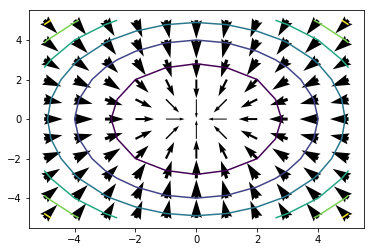
\includegraphics[width=0.4\linewidth,keepaspectratio]{diff12}
\end{center}
\begin{itemize}
\item The arrows in the plot point in the direction of the gradient.
\item The width of the arrows is proportional to the value of the gradient. The width of the arrows and the gradient decreases as function gets closer to the minimum. If this is the case everywhere, you can say that a function is convex. It is always much easier to find minimum of convex functions.
\item The direction of the gradient is always perpendicular to the contours. 
\end{itemize}

\end{frame}


%%%%%%%%%%%%%%%%%%%%%%%%%%%%%%%%%%%%%%%%%%%%%%%%%%%%%%%%%%%%%%%%%%%%%%%%%%%%%%%%%%
\begin{frame}[fragile]\frametitle{}
\begin{center}
{\Large Linear Approximation}
\end{center}
\end{frame}




%%%%%%%%%%%%%%%%%%%%%%%%%%%%%%%%%%%%%%%%%%%%%%%%%%%%%%%%%%%

\begin{frame}[fragile]  \frametitle{Linear Approximation}
  \textbf{Definition}
    Suppose that $f$ has continuous partial derivatives.  We define the \underline{linearization of $f$ at $(x_0,y_0)$} as
    $$
      L(x,y) = f(x_0,y_0) +  f_x(x_0,y_0)(x-x_0) + f_y(x_0,y_0)(y-y_0).
    $$
    The function $L$ is also called the linear approximation or tangent plane approximation of $f$ near $(x_0,y_0)$.
    
  
  \textbf{Example}
    Approximate the value of $3x^2+5y^2$ at $(1.01,1.01)$.
  
  
\end{frame}


%%%%%%%%%%%%%%%%%%%%%%%%%%%%%%%%%%%%%%%%%%%%%%%%%%%%%%%%%%%
\begin{frame}[fragile]\frametitle{}
  \textbf{Definition}
    The function $z=f(x,y)$ is  \underline{differentiable} at $(a,b)$ if the quantity $\Delta z = f(a+\Delta x,b+\Delta y) -f(a,b)$ can be expressed as
    $$
      \Delta z = f_x(a,b)\Delta x + f_y(a,b)\Delta y +\epsilon_1\Delta x + \epsilon_2\Delta y
    $$
    where $\epsilon_1,\epsilon_2 \rightarrow 0$ as $(\Delta x,\Delta y)\rightarrow (0,0)$.
   
  
  \textbf{Theorem}
    If $f_x$ and $f_y$ are defined and continuous near $(a,b)$, then $f$ is differentiable at $(a,b)$.
  
\end{frame}

%%%%%%%%%%%%%%%%%%%%%%%%%%%%%%%%%%%%%%%%%%%%%%%%%%%%%%%%%%%
\begin{frame}[fragile]\frametitle{}
  \textbf{Example}
    Show that $f(x,y)=y\sin(xy)$ is differentiable at $(\frac{1}{2},\pi)$.  Find its linearization at $(\frac{1}{2},\pi)$ and use it to 
    approximate $f(.55,3)$.
    
  
  \textbf{Definition}
    Given a function $f(x,y)$, we define \underline{differentials} $dx$ and $dy$ to be independent variables.  We define the \underline{total differential} $\text{dz}$ as
    $$ \text{dz} = f_x(x,y)\text{dx} + f_y(x,y)\text{dy}.$$
   
  
  \textbf{Note}
    In the above expression, the dependent variable $\text{dz}$ depends on the 4 independent variables $x,y,\text{dx}$ and $\text{dy}$.
   
  
   \textbf{Note}
    If $f$ has continuous partials, then $f(x+\text{dx},y+\text{dy})\approx f(x,y) +\text{dz}$.
  

\end{frame}


%%%%%%%%%%%%%%%%%%%%%%%%%%%%%%%%%%%%%%%%%%%%%%%%%%%%%%%%%%%
\begin{frame}[fragile]\frametitle{}
\textbf{Example}
Suppose that we are to construct a cylindrical water tank with radius 2m and height 1m.  Suppose also that we can ensure that the radius and height of the tank are correct to within 1mm.  What is the maximum error in the volume of the tank.
 

\textbf{Fact}
If $f(\vec{x})$ is a real valued function of $n$ variables, then we consider the differentials $\text{dx}_i$ as independent variables and define the total differential to be 
$$ \text{dz} = \sum_{i=1}^n f_{x_i}(\vec{x})\text{dx}_i.$$ 
If $f$ is differentiable, then it will be true that 
$$f(\vec{x}+\vec{\text{dx}})\approx f(\vec{x})+\text{dz}.$$

\end{frame}



%%%%%%%%%%%%%%%%%%%%%%%%%%%%%%%%%%%%%%%%%%%%%%%%%%%%%%%%%%%
\begin{frame}[fragile]\frametitle{}
\textbf{Theorem}[Chain Rule - Case 1]
Suppose that $z=f(x,y)$ is a differentiable function and that $x(t)$ and $y(t)$ are both differentiable functions as well.  Then,
$$
  \text{dz}dt = \frac{\partial f}{\partial x} \text{dx}dt + \frac{\partial f}{\partial y}\text{dy}dt.
$$
  

\textbf{Example}
Suppose that $z=xy^2 + 5x^3y$ where $x(t)=e^t$ and $y(t)=\sin(t)$.  Find $\text{dz}dt$ when $t=0$.
  

\textbf{Example}
The pressure (in kilopascals kPa), volume (in liters L) and temperature (in kelvins K) of an ideal gas are related by the equation $PV=8.31 T$.  Find the rate at which the pressure is changing when the temperature is 300 K and increasing at a rate of 0.1 K/s and the volume is 100 L and increasing at 0.2 L/s.

\end{frame}


%%%%%%%%%%%%%%%%%%%%%%%%%%%%%%%%%%%%%%%%%%%%%%%%%%%%%%%%%%%
\begin{frame}[fragile]\frametitle{}
\textbf{Theorem}[Chain Rule - Case 2]
Suppose that $z=f(x,y)$ is a differentiable function of $x$ and $y$, where $x(s,t)$ and $y(s,t)$ are also differentiable functions.  Thesn
$$
\frac{\partial z}{\partial s} = \frac{\partial z}{\partial x}\frac{\partial x}{\partial s} + \frac{\partial z}{\partial y}\frac{\partial y}{\partial s} 
\quad\mbox{and}\quad
\frac{\partial z}{\partial t} = \frac{\partial z}{\partial x}\frac{\partial x}{\partial t} + \frac{\partial z}{\partial y}\frac{\partial y}{\partial t}
$$
 

\textbf{Example}
Suppose that $z=\cos(x)\sin(y)$ and $x(s,t)= st$ and $y(s,t)=s^2t$.  Compute the partial derivatives of $z$ with respect to $s$ and $t$.

\end{frame}


%%%%%%%%%%%%%%%%%%%%%%%%%%%%%%%%%%%%%%%%%%%%%%%%%%%%%%%%%%%
\begin{frame}[fragile]\frametitle{}
\textbf{Theorem}[Chain Rule - General Version]
Suppose that $u$ is a differentiable function in the variables $x_1,x_2,\dots, x_n$ and each $x_i$ is a differentiable function of the variables $t_1,t_2,\dots,t_m$.  Then,
$$
\frac{\partial u}{\partial t_i} = \sum_{j=1}^n \frac{\partial u}{\partial x_j} \frac{\partial x_j}{\partial t_i}.
$$
  

\textbf{Example}
Suppose that $u=x^3y+y^3z +z^3x$ where $x=rs\sin(t)$, $y=rs\cos(t)$ and $z=rse^t$.  Find $\frac{\partial u}{\partial s}$. 

\end{frame}



%%%%%%%%%%%%%%%%%%%%%%%%%%%%%%%%%%%%%%%%%%%%%%%%%%%%%%%%%%%
\begin{frame}[fragile]\frametitle{Implicit Differentiation}
Given an equation $F(x,y)=0$, we suppose that this equation implicitly defines $y$ as a function of $x$.  \\ 
Applying the chain rule gives 
\begin{eqnarray*}
 \frac{\partial F}{\partial x} \frac{\text{dx}}{\text{dx}} + \frac{\partial F}{\partial y}\text{dy}dx  &=& 0\\  
  \Rightarrow  \text{dy}dx &=& \frac{\frac{-\partial F}{\partial x}}{\frac{\partial F}{\partial y}} =\frac{-F_x}{F_y}
\end{eqnarray*}  

\textbf{Example}
Find the slope of the line tangent to the unit circle at the point $(\frac{\sqrt{2}}{2}, \frac{\sqrt{2}}{2})$.

\end{frame}


%%%%%%%%%%%%%%%%%%%%%%%%%%%%%%%%%%%%%%%%%%%%%%%%%%%%%%%%%%%
\begin{frame}[fragile]\frametitle{}
Now suppose that $z$ is given implicitly as a function of $x$ and $y$ by the equation 
\begin{eqnarray*}
F(x,y,z)&=&0  \\ 
\Rightarrow F(x,y,f(x,y))&=&0 \\  
\Rightarrow  \frac{\partial F}{\partial x} \frac{\partial x}{\partial x} + \frac{\partial F}{\partial y}\frac{\partial y}{\partial x}  
                                                      +  \frac{\partial F}{\partial z} \frac{\partial z}{\partial x} &=& 0\\  
    \Rightarrow  \frac{\partial F}{\partial x}   +  \frac{\partial F}{\partial z} \frac{\partial z}{\partial x} &=& 0\\  
    \Rightarrow  \frac{\partial z}{\partial x} &=& \frac{-  \frac{\partial F}{\partial x}}{\frac{\partial F}{\partial z}}  \\
                                                                 &=&\frac{-F_x}{F_z}                    
\end{eqnarray*}  
\end{frame}


%%%%%%%%%%%%%%%%%%%%%%%%%%%%%%%%%%%%%%%%%%%%%%%%%%%%%%%%%%%
\begin{frame}[fragile]\frametitle{}
\textbf{Implicit Differentiation}
Suppose that $x$, $y$ and $z$ satisfy the equation $F(x,y,z)=0$ where $F$ is differentiable then under the assumption that $z$ is implicitly defined as a differentiable function of $x$ and$y$, we obtain the formulas
\begin{eqnarray*}
\frac{\partial z}{\partial x} &=& \frac{-  \frac{\partial F}{\partial x}}{\frac{\partial F}{\partial z}}  \\
\frac{\partial z}{\partial y} &=& \frac{-  \frac{\partial F}{\partial y}}{\frac{\partial F}{\partial z}}
\end{eqnarray*}
  

\textbf{Example}
Recall that the equation of the unit sphere is given by $x^2+y^2+z^2=1$.  Use implicit differentiation to find the equation of the tangent plane at the point $\left(\frac{\sqrt{3}}{3}, \frac{\sqrt{3}}{3}, \frac{\sqrt{3}}{3} \right)$

\end{frame}



%%%%%%%%%%%%%%%%%%%%%%%%%%%%%%%%%%%%%%%%%%%%%%%%%%%%%%%%%%%
\begin{frame}[fragile]\frametitle{}
\textbf{Definition}
We define the \underline{directional derivative} of the function $f(x,y)$ at the point $(x_0,y_0)$ in the direction of the unit vector 
$u=(a,b)$ ($u$ should be thought of as a vector in the $xy$-plane) as
$$
  D_u f(x_0,y_0) = \lim_{h\rightarrow 0} \frac{f(x_0+ah,y_0+bh)-f(x_0,y_0)}{h}.
$$
  

\textbf{Theorem}
If $f(x,y)$ is differentiable, then 
$$
D_u f(x,y) = f_x(x,y)a+f_y(x,y)b.
$$

\end{frame}



%%%%%%%%%%%%%%%%%%%%%%%%%%%%%%%%%%%%%%%%%%%%%%%%%%%%%%%%%%%
\begin{frame}[fragile]\frametitle{}
\textbf{Proof}
Define $g(h) = f(x_0+ah,y_0+bh)$.    \\ 
Then, we have that   \\
\begin{eqnarray*}
g'(0)&=& \lim_{h\rightarrow 0}\frac{g(h)-g(0)}{h} =
        \lim_{h\rightarrow 0}\frac{f(x_0+ah,y_0+bh)-f(x_0,y_0)}{h} \\ 
        &=&D_u f(x_0,y_0).
\end{eqnarray*}  
We can also write $g(h)=f(x,y)$ where $x=x_0+ah$ and $y=y_0+bh$.  \\ 
Applying the chain rule, we have,
$$
g'(h)=f_x(x,y)a+f_y(x,y)b.
$$ 
Thus, 
$$
D_u f(x_0,y_0)= g'(0) = f_x(x_0,y_0)a+f_y(x_0,y_0)b.
$$

\end{frame}


%%%%%%%%%%%%%%%%%%%%%%%%%%%%%%%%%%%%%%%%%%%%%%%%%%%%%%%%%%%
\begin{frame}[fragile]\frametitle{}
\textbf{Note}
  If the vector $u$ is at an angle $\theta$ with the $x$-axis then we can write $u=(\cos(\theta),\sin(\theta))$.  Thus
  $$
    D_u f(x,y) = f_x(x,y)\cos(\theta) + f_y(x,y)\sin(\theta).
  $$


\textbf{Example}
Find the directional derivative $D_u f(x,y)$ of the function $f(x,y)=x^2+xy+y^2$ in the direction of the unit vector which is at an angle of $\theta=\frac{\pi}{3}$ to the $x$-axis.

\end{frame}


%%%%%%%%%%%%%%%%%%%%%%%%%%%%%%%%%%%%%%%%%%%%%%%%%%%%%%%%%%%
\begin{frame}[fragile]\frametitle{}
\textbf{Note}
The directional derivative of $f$ in the direction of $u$ can be written as
$$
D_u f(x,y) = (f_x(x,y), f_y(x,y)) \cdot u.
$$
  

\textbf{Definition}
We define the \underline{gradient} of a function $f(x,y)$ as
$$
\nabla f = (f_x(x,y), f_y(x,y)) = f_x(x,y)i + f_y(x,y)j.
$$
  

\textbf{Fact}
If $u$ is a unit vector and $f(x,y)$ is a function of 2 variables then
$$
D_u f(x,y) = \nabla f \cdot u.
$$

\end{frame}



%%%%%%%%%%%%%%%%%%%%%%%%%%%%%%%%%%%%%%%%%%%%%%%%%%%%%%%%%%%
\begin{frame}[fragile]\frametitle{}
\textbf{Example}
Consider the function $f(x,y)=e^{xy}$. Compute the gradient of $f$.  Compute the directional derivative of $f$ in the direction of $u=(\sqrt{3}/2,1/2)$.

\end{frame}



%%%%%%%%%%%%%%%%%%%%%%%%%%%%%%%%%%%%%%%%%%%%%%%%%%%%%%%%%%%
\begin{frame}[fragile]\frametitle{Functions of 3 variables}
 
\textbf{Definition}
 The \underline{directional derivative} of $f(x,y,z)$ at $(x_0,y_0,z_0)$ in the direction of the unit vector $u=(a,b,c)$ is
 $$
   D_u f(x_0,y_0,z_0) = \lim_{h\rightarrow 0} \frac{f(x_0+ah,y_0+bh,z_0+ch)-f(x_0,y_0,z_0)}{h}.
 $$
 if this limit exists.
 

\textbf{Fact}
 If $f(x,y,z)$ is differentiable then
 $$
 D_u f(x,y,z) = f_x(x,y,z)a +f_y(x,y,z)b + f_z(x,y,z)c.
 $$
 
\end{frame}


%%%%%%%%%%%%%%%%%%%%%%%%%%%%%%%%%%%%%%%%%%%%%%%%%%%%%%%%%%%
\begin{frame}[fragile]\frametitle{}
\textbf{Definition}
 We define the \underline{gradient} of $f(x,y,z)$ as
 $$
 \nabla f = (f_x,f_y,f_z).
 $$
 

\textbf{Fact}
 $$
 D_u f(x,y,z) = \nabla f(x,y,z) \cdot u
 $$
  

\textbf{Example}
 Suppose that $f(x,y,z) = sin(xy)e^z$.  Compute $\nabla f$.  What is the directional derivative at $(\pi,1/2,0)$ in the direction $(\sqrt{3}/3, \sqrt{3}/3, \sqrt{3}/3)$.  Can you find the direction which maximizes $D_u f$ at this point?

\end{frame}


%%%%%%%%%%%%%%%%%%%%%%%%%%%%%%%%%%%%%%%%%%%%%%%%%%%%%%%%%%%
\begin{frame}[fragile]\frametitle{}
\textbf{Theorem}
 Suppose that $f$ is a differentiable function of two or three variables.  The maximal value of the directional derivative $D_u f(\vec{x})$ at the point $\vec{x}$ is $|\nabla f|$ and it occurs when $u= \frac{1}{|\nabla f|} \nabla f$.
  

\textbf{Example}
 Consider the function $f(x,y,z) = e^{xyz}$.  What is the directional derivative at the point $(0,1,0)$ in the direction of 
 $\overrightarrow{((0,1,0),(1,1,1))}$.  What is the maximum value of the directional derivative at this point?  In which direction does it occur?

\end{frame}



%%%%%%%%%%%%%%%%%%%%%%%%%%%%%%%%%%%%%%%%%%%%%%%%%%%%%%%%%%%
\begin{frame}[fragile]\frametitle{Tangent Planes to Level Surfaces}
Suppose that $S$ is the level surface of $F(x,y,z)$ given by $F(x,y,z)=k$ and $P=(x_0,y_0,z_0)$ is a point on $S$.  \\ 
Let $C$ be any curve that lies on $S$ and passes through $P$.  \\ 
Then $C$ can be parametrized by $r(t)=(x(t),y(t),z(t))$.  \\ 
Suppose that $r(t_0)=P$.  \\ 
Note that $F(x(t),y(t),z(t))= k$ because $C$ lies on $S$.  \\ 
Supposing all functions to be differentiable, we can use the chain rule to obtian,
$$
0 = F_x x'(t) + F_y y'(t) + F_z z'(t) =  \nabla F \cdot r'(t).
$$ 
That is, $\nabla F(P)$ is orthogonal to the tangent vector at $P$ of any curve along $S$ passing through $P$. 
\end{frame}



%%%%%%%%%%%%%%%%%%%%%%%%%%%%%%%%%%%%%%%%%%%%%%%%%%%%%%%%%%%
\begin{frame}[fragile]\frametitle{}
\textbf{Definition}
 We define the \underline{tangent plane to the level surface $F(x,y,z)=k$} \underline{at $P=(x_0,y_0,z_0)$} as the plane that passes through $P$ and has normal vector $\nabla F(x_0,y_0,z_0)$.  This plane has equation
 $$
   F_x(x_0,y_0,z_0) (x-x_0) + F_y(x_0,y_0,z_0) (y-y_0) + F_z(x_0,y_0,z_0) (z-z_0) = 0.
 $$ 
 or 
 $$
 \nabla F(x_0,y_0,z_0) \cdot \overrightarrow{(P,(x,y,z))}  = 0
 $$
 
\end{frame}



%%%%%%%%%%%%%%%%%%%%%%%%%%%%%%%%%%%%%%%%%%%%%%%%%%%%%%%%%%%
\begin{frame}[fragile]\frametitle{}
\textbf{Definition}
 We define the \underline{normal line} to the level surface $F(x,y,z)=k$ at $P$ to be the line passing through $P$ and orthogonal to the tangent plane,  that is the line through $P$ parallel to the normal vector for the tangent plane which is $\nabla F(P)$.  This line has symmetric equations
 $$
   \frac{x-x_0}{F_x(x_0,y_0,z_0)} = \frac{y-y_0}{F_y(x_0,y_0,z_0)} = \frac{z-z_0}{F_z(x_0,y_0,z_0)}.
 $$
 
\end{frame}


%%%%%%%%%%%%%%%%%%%%%%%%%%%%%%%%%%%%%%%%%%%%%%%%%%%%%%%%%%%
\begin{frame}[fragile]\frametitle{}
\textbf{Note}
 We can think of the graph $z=f(x,y)$ of $f(x,y)$ as the level surface $F(x,y,z)=0$ where $F(x,y,z)=f(x,y)-z$. \\ 
 In this case, $\nabla F = (f_x,f_y,-1)$  \\ 
 So the tangent plane to the graph of $f$ as a level surface at $P$ would have equation 
 $$
  f_x(x_0,y_0,z_0) (x-x_0) + f_y(x_0,y_0,z_0) (y-y_0) - (z-z_0) = 0.
$$
 which is consistent with our previous definition of tangent plane.  \\ 
 The normal line has equation
 $$
   \frac{x-x_0}{f_x(x_0,y_0,z_0)} = \frac{y-y_0}{f_y(x_0,y_0,z_0)} = -(z-z_0).
 $$

\end{frame}


%%%%%%%%%%%%%%%%%%%%%%%%%%%%%%%%%%%%%%%%%%%%%%%%%%%%%%%%%%%
\begin{frame}[fragile]\frametitle{}
 \textbf{Example}
 Find the equations of the tangent plane and normal line at the point $(3,2,2)$ to the ellipsoid $\frac{x^2}{9} + \frac{y^2}{4} + z^2 = 6$.

\end{frame}

